\documentclass{article}
\usepackage[english,brazilian]{babel}
\usepackage[utf8]{inputenc}
\usepackage{fancyhdr}
\usepackage{hyperref}
\usepackage{mathtools}
\usepackage[shortlabels]{enumitem}
\usepackage{changepage}
\usepackage{float}

\hypersetup{
    colorlinks=true,
    linkcolor=cyan,
    urlcolor=cyan}

\title{Modelagem de um sistema dinâmico planta-herbívoro levando em conta a presença de plantas tóxicas no ambiente}
\author{André Ribeiro, Erlon Kelvim}
\date{\today}

\renewcommand*\contentsname{Sumário}

\begin{document}

\maketitle

\newpage

\tableofcontents

\newpage

\section{Introdução}

Embora o estudo da relação entre herbívoros-plantas já seja estudado a muitos anos, apenas a pouco tempo começou-se as pesquisas sobre a influência da toxidade das plantas sobre tal relação. Nosso trabalho busca usar como base empírica a relação mamífero-planta a fim criar um modelo matemático em que o efeito negativo gerado pela toxidade das plantas seja expresso de maneira mais explícita em nosso modelo \cite{LI} \cite{FENG}.

O modelo mais usado para análise da relação mamífero-planta é o Holling tipo II \cite{CRAWFORD}\cite{HOLLING} que foi proposto em um sistema onde haja uma abundância de presas (plantas) e a reação do predador a tal sistema e chegou-se que a resposta funcional seria um aumento do consumo da presa a medida que sua biomassa aumenta, até a capacidade do predador de comer a presa esteja saciada, a partir disso, independente do aumento da biomassa da presa o consumo do predador se manterá constante. Entretanto a existência de toxinas nas plantas pode alterar esse sistema \cite{ZHILAN}, pois a variação da toxidade das plantas faz com que os mamíferos se alimentem seletivamente, fazendo com que a diversidade da vegetação e os processos do ecossistema sejam afetados.


\section{Metodologia}

Inicialmente, consideramos o sistema mais simples possível, onde há somente uma planta e não há toxicidade. Seja $n$ o número de galhos de plantas disponíveis no sistema, $t_b$ o tempo necessário para um herbívoro encontrar o galho, $r$ a taxa de crescimento por unidade de galho e $t_h$ o tempo (em segundos) que um herbívoro leva para consumir e digerir uma unidade de galho. Com essas informações, temos que o total de galhos encontrados em um dado tempo $t_b$ é $T_g = n r t_b$ e o tempo total gasto pelo herbívoro consumindo galhos é $T_h = t_h n r t_b = t_h T_g$. Definimos então a taxa de consumo
\begin{equation}
    f(n) \coloneqq \frac{T_g}{t_b + T_h} = \frac{n r}{1 + t_h n r}
\end{equation}
Note que da maneira como $t_h$ foi definido, temos que $h_{\max} = \frac{1}{t_h}$ é o número máximo de galhos que um herbívoro pode consumir por unidade de tempo, na ausência de toxicidade. Note também que
\begin{equation}
    h_{\max} = \lim_{n \to \infty} f(n)
\end{equation}
i.e. $h_{\max}$ é assintota da função $f$. Contudo, nossa análise até aqui considerava o sistema incompleto, sem toxicidade. Na presença dessa nova variável, devemos ter uma taxa real de consumo $\eta(n)$ menor que $f(n)$ e uma quantidade máxima de galhos contendo toxinas $H_{\max}$ menor que $h_{\max}$. Para encontrar a função $\eta$, note que a função $R = \frac{\eta}{f}$ deve ser uma função decrescente de $f$, com $R \to 1$ quando $f \to 0$, já que se o consumo está diminuindo, o consumo de plantas com toxicidade está aumentando, e se $\frac{H_{\max}}{\alpha}$ é um valor limitante para $f$, $R \to 0$ quando $f \to \frac{H_{\max}}{\alpha}$, já que há plantas em abundância e a taxa de consumo de plantas com toxicidade diminui. Uma boa maneira de expressar essas propriedades é considerar $R$ como a seguinte função linear \[ R = 1 - \frac{\alpha f}{H_{\max}} \] onde a constante de proporção $\alpha$ é escolhida de modo que $\max\{\eta\} = H_{\max}$. Lembrando que $R = \frac{\eta}{f}$, temos que
\begin{equation*}
    \frac{\eta}{f} = 1 - \frac{\alpha f}{H_{\max}}
\end{equation*}
logo
\begin{equation}
    \eta(f) = f\left(1 - \frac{\alpha f}{H_{\max}}\right)
\end{equation}
Para encontrar o valor de $\alpha$, vamos encontrar o máximo da função $\eta$
\begin{equation*}
    \eta' = f'\left(1 - \frac{2 \alpha f}{H_{\max}}\right) \\
\end{equation*}
Como buscamos $\eta' = 0$, devemos ter $f' = 0 \quad \lor \quad 1 - \frac{2 \alpha f}{H_{\max}} = 0$. O primeiro caso ocorre apenas quando $n \to \infty$, iremos então considerar o segundo caso
\begin{align*}
    1 - \frac{2 \alpha f}{H_{\max}} &= 0 \\
    \frac{2 \alpha f}{H_{\max}} &= 1 \\
    \frac{H_{\max}}{2\alpha} &= f
\end{align*}
Substituindo o valor que maximiza a função $\eta$ obtemos
\begin{align*}
    \eta\left(\frac{H_{\max}}{2\alpha}\right) &= \frac{H_{\max}}{2\alpha}\left(1 - \frac{\alpha \cdot \frac{H_{\max}}{2\alpha}}{H_{\max}} \right) \\
                                                &= \frac{H_{\max}}{2\alpha} \cdot \frac{1}{2} \\
                                                &= \frac{H_{\max}}{4\alpha} 
\end{align*}
Havíamos escolhido $\alpha$ de modo que $\max\{\eta\} = H_{\max}$, então $\alpha = \frac{1}{4}$. Como $\eta$ é a taxa de consumo, faz sentido considerar apenas o intervalo de definição para o qual $\eta \geq 0$, ou seja
\begin{equation*}
    \eta \geq 0\;\Longrightarrow\;f\left(1 - \frac{f}{4H_{\max}}\right) \geq 0 \\
\end{equation*}
Já que $f > 0$, devemos ter
\begin{align*}
    1 - \frac{f}{4H_{\max}} \geq 0\;\Longrightarrow\;1 \geq \frac{f}{4H_{\max}}\;\Longrightarrow\;4H_{\max} \geq f
\end{align*}
Por (2), obtemos
\begin{align*}
    4H_{\max} \geq f \quad \land \quad f < h_{\max}\;\Longrightarrow\;4H_{\max} > h_{\max}\;\Longrightarrow\;H_{\max} > \frac{h_{\max}}{4}
\end{align*}
Temos então a seguinte relação entre a quantidade máxima de galhos contendo toxinas consumidas por um herbívoro e a quantidade máxima de galhos consumidas por um herbívoro
\begin{equation}
    \frac{h_{\max}}{4} < H_{\max} < h_{\max}
\end{equation}
Com isso, temos o seguinte sistema de EDO's que descreve nosso sistema
\begin{align*}
    \frac{dn}{dt} &= rn\left( 1 - \frac{n}{W} \right) - \eta(n)X \\
    \frac{dX}{dt} &= Y\eta(n)X - XZ
\end{align*}
onde $X = X(t)$ representa a quantidade de herbívoros no tempo $t$, $Y$  a conversão da biomassa de espécies de plantas consumidas em novos herbívoros, Z a taxa de morte per capita de herbívoros devido a causas não relacionadas à toxicidade da planta e $W$ a capacidade de carregamento do herbívoro. \\

Podemos obter a taxa real de consumo como uma função da abundância de plantas no sistema substituindo a equação (1) na equação (3)
\begin{align}
    \eta(n) &= f(n)\left(1 - \frac{f(n)}{4H_{\max}}\right) \nonumber \\
            &= \frac{n r}{1 + t_h n r} \left( 1 - \frac{n r}{4H_{\max}(1 + t_h n r)} \right)
\end{align}
Para generalizar o modelo obtido, consideramos os vetores $n = (n_1,n_2,\cdots,n_k)$, $r = (r_1,r_2,\cdots,r_k)$, $t_h = (t_{h_1},t_{h_2},\cdots,t_{h_k})$ e $H_{\max} = (H_{\max_1}, H_{\max_2},\cdots,H_{\max_k})$, onde cada componente é relativo à planta da espécie $i$, e cada $r_i$ é considerado em um ambiente em que não há competição de recursos pelas plantas. Podemos então obter $f = (f_1,f_2,\cdots,f_k)$ e $\eta = (\eta_1,\eta_2,\cdots,\eta_k)$, onde cada componente é dada por
\begin{equation}
    f_i(n) = \frac{n_i r_i}{1 + \sum_{i=1}^{k} t_{h_i} n_i r_i}
\end{equation}
e
\begin{equation}
    \eta_i(n)  = f_i(n)\left(1 - \frac{f_i(n)}{4H_{\max_i}}\right)
\end{equation}
Utilizando a equação acima, nosso modelo para o sistema planta-herbívoro é descrito pelo seguinte sistema de EDO's
\begin{equation}
\begin{aligned}
    \frac{dn_i}{dt} &= g_i n_i \left( 1 - \frac{n_i + \sum_{\overset{j=1}{j \neq i}}^k \beta_{ij}n_j}{W_i} \right) - \eta_i(n)X \\
    \frac{dX}{dt}   &= \sum_{j=1}^k Y_j\eta_j(n)X - XZ
\end{aligned}
\end{equation}
onde $\beta_{ij}$ é o parâmetro de competição dos herbívoros, que mede a intensidade de competição da espécie $j$ contra a espécie $i$. Todos os parâmetros estão definidos na tabela abaixo, para alguns tipos de planta. Note que para cada $i$ (espécie), os valores que acima possuem esse índice podem variar em relação aos valores abaixo
\begin{table}[h!]
    \begin{tabular}{|c|p{9cm}|r|} \hline
    Parâmetro  & Unidade & Valor (ou intervalo) \\ \hline
    $t_b$ & Taxa de encontro por unidade de galho & [0.0001,0.0005] \\
    $g_i$ & Máximo de novas unidades de galhos/galho por dia & [0.003,0.01] \\
    $t_h$ & Tempo para consumir uma unidade de galho na ausência de toxinas & [0.0025,0.03125] \\
    $W$ & Capacidade de carga & $[10^4,10^5]$ \\
    $Y$ & Constante de conversão (herbívoro/unidade de galho) & [0.00003,0.00006] \\
    $Z$ & Taxa de morte de herbívoros per capita &  [0.00003,0.0002] \\
    $H_{\max}$ & Máximo de unidades de galho contendo toxina (de um certo tipo) que um herbívoro pode consumir por dia & [8,80] \\
    $\beta$ & Coeficiente de competição & $[10^{-1},10]$ \\ \hline
    \end{tabular}
    \caption{Parâmetros, unidades e valores das variáveis para algumas espécies de plantas}
    \label{tab:my_label}
\end{table}

\newpage

\section{Equilíbrio e estabilidade}

\subsection{Equilíbrios de fronteira}

Iremos considerar um sistema com duas espécies ($i = 1,\:2$) na qual

\begin{equation}
    H_{\max_i} = \frac{h_{\max_i}}{2}
\end{equation}

Temos que a função $f(n)$ é monótona crescente, pois

\begin{equation*}
    f'(n) = \frac{r}{(1 + t_hnr)^2} > 0
\end{equation*}

e

\begin{equation*}
    f(n_1) > f(n_2) \iff \frac{n_1r}{1 + t_hn_1r} > \frac{n_2r}{1 + t_hn_2r} \iff n_1(1 + t_hn_2r) > n_2(1 + t_hn_1r) \iff n_1 > n_2
\end{equation*}

Portanto a função $\eta_i(n)$ é monótona crescente, com assíntota $H_{\max_i}$:

\begin{align*}
    \lim_{n \to \infty} \eta_i(n) &= \lim_{n \to \infty} f_i(n)\left(1 - \frac{f_i(n)}{4H_{\max_i}}\right) \\
                                  &= h_{\max_i}\left( 1 - \frac{h_{\max_i}}{4H_{\max_i}} \right) \\
                                  &= h_{\max_i} - \frac{h_{\max_i}^2}{2h_{\max_i}} \\
                                  &= \frac{h_{\max_i}}{2}
\end{align*}

Vamos agora encontrar os equilíbrios de fronteira do sistema em (8). Se $X = 0$, então

\begin{align*}
    \begin{cases}
    g_1 n_1 \left( 1 - \frac{n_1 + \beta_{12}n_2}{W_1} \right) = 0 \vspace{2mm} \\
    g_2 n_2 \left( 1 - \frac{n_2 + \beta_{21}n_1}{W_2} \right) = 0
    \end{cases} \iff \quad
    \begin{aligned}
    g_1 n_1 = 0 \quad \lor \quad 1 - \frac{n_1 + \beta_{12}n_2}{W_1} = 0 \\
    g_2 n_2 = 0 \quad \lor \quad 1 - \frac{n_2 + \beta_{21}n_1}{W_2} = 0
    \end{aligned}
\end{align*}

É imediato que $n_1 = n_2 = 0$ é uma solução (trivial) do sistema acima - portanto há um equilíbrio na origem. Consideremos agora $n_1 \neq 0,\:n_2 = 0$. Então

\begin{align*}
    1 - \frac{n_1 + \beta_{12}n_2}{W_1} = 0 \iff n_1 = W_1
\end{align*}

Portanto $(0,W_1,0)$ é uma solução. Por simetria, temos que $(0,0,W_2)$ também é solução. Para o caso $n_1,\:n_2 \neq 0$, temos

\begin{align*}
    \begin{cases}
    1 - \frac{n_1 + \beta_{12}n_2}{W_1} = 0 \\
    1 - \frac{n_2 + \beta_{21}n_1}{W_2} = 0
    \end{cases} \iff
    \begin{cases}
    n_1 + \beta_{12}n_2 = W_1 \\
    n_2 + \beta_{21}n_1 = W_2
    \end{cases}
\end{align*}

\begin{align*}
    n_1 = W_1 - \beta_{12}n_2 &\implies n_2 + \beta_{21}(W_1 - \beta_{12}n_2) = W_2 \\\\
    &\implies n_2 = \frac{W_2 - \beta_{21}W_1}{1 - \beta_{12}\beta_{21}} \quad \land \quad n_1 = \frac{W_1 - \beta_{12}W_2}{1 - \beta_{12}\beta_{21}}
\end{align*}

Chamando de $\Bar{n}_1$ e $\Bar{n}_2$ as soluções encontradas, temos que $(0,\Bar{n}_1,\Bar{n}_2)$ é ponto de equilíbrio. Assumimos agora que $X \neq 0$. Calcularemos o caso $n = (n_1,0)$, o caso $n = (0,n_2)$ é simétrico. Como $X$ não é nulo, voltamos à equação $\frac{dX}{dt} = 0$

\begin{align}
    \sum_{j=1}^2 Y_j\eta_j(n)X - XZ = 0 &\implies Y_1\eta_1(n) = Z \\
                                        &\implies Y_1\left[f_1(n)\left(1 - \frac{f_1(n)}{4H_{\max_1}}\right)\right] = Z \nonumber \\
                                        &\implies \frac{[f_1(n)]^2}{4H_{\max_1}} - f_1(n) + \frac{Z}{Y_1} = 0 \nonumber \\
                                        &\implies f_1(n) = 2H_{\max_1}\left(1 \pm \sqrt{1 - \frac{Z}{Y_1H_{\max_1}}} \right) \nonumber
\end{align}


Notemos que, como $h_{\max_1}$ é assíntota de $f_1(n)$, temos por $(9)$ que \linebreak $f_1(n) < 2H_{\max_1}$ e portanto

\begin{equation}
    f_1(n) = 2H_{\max_1}\left(1 - \sqrt{1 - \frac{Z}{Y_1H_{\max_1}}} \right)
\end{equation}

Notemos também que

\begin{align*}
    f_1(n) = f_1(n_1,0) = \frac{n_1r_1}{1 + t_{h_1}r_1n_1}
\end{align*}

substituindo em (11)

\begin{align*}
    \frac{n_1r_1}{1 + t_{h_1}r_1n_1} = 2H_{\max_1}\left(1 - \sqrt{1 - \frac{Z}{Y_1H_{\max_1}}} \right) \\
    n_1\left( \sqrt{1 - \frac{Z}{Y_1H_{\max_1}}} \right) = \frac{2H_{\max_1}}{r_1}\left(1 - \sqrt{1 - \frac{Z}{Y_1H_{\max_1}}} \right) \\
    n_1 = \frac{2H_{\max_1}}{r_1}\left( \frac{1}{\sqrt{1 - \frac{Z}{Y_1H_{\max_1}}}} - 1 \right)
\end{align*}

Chamemos o valor encontrado acima de $\tilde{n}_1$. Podemos então encontrar $X$ por meio da equação $\frac{d\tilde{n}_1}{dt} = 0$

\begin{align*}
    g_1\tilde{n}_1\left( 1 - \frac{\tilde{n}_1}{W_1} \right) = \eta_1(n)X 
\end{align*}

Por $(10)$, temos que $\eta_1(n) = \frac{Z}{Y_1}$, portanto

\begin{align*}
    X = \frac{Y_1g_1\tilde{n}_1}{Z}\left( 1 - \frac{\tilde{n}_1}{W_1} \right)
\end{align*}

Seja $\tilde{X}$ a solução acima. Temos então um equilíbrio em $(\tilde{X},\tilde{n}_1,0)$. O outro equilíbrio está em $(\hat{X},0,\hat{n}_2)$, onde

\begin{align*}
    \hat{n}_2 &= \frac{2H_{\max_2}}{r_2}\left( \frac{1}{\sqrt{1 - \frac{Z}{Y_2H_{\max_2}}}} - 1 \right) \\
    \hat{X} &= \frac{Y_2g_2\hat{n}_2}{Z}\left( 1 - \frac{\hat{n}_2}{W_2} \right)
\end{align*}

Temos então os seguintes equilíbrios de fronteira

\begin{align*}
    &E_0 = (0,0,0) \quad E_1 = (0,W_1,0) \quad E_2 = (0,0,W_2) \\
    &\Bar{E} = (0,\Bar{n}_1,\Bar{n}_2) \quad \tilde{E} = (\tilde{X},\tilde{n}_1,0) \quad \hat{E} = (\hat{X},0,\hat{n}_2)
\end{align*}

Utilizando \textit{SageMath9.3} para visualizar os 4 primeiros equilíbrios:

\begin{figure}[H]
    \centering
    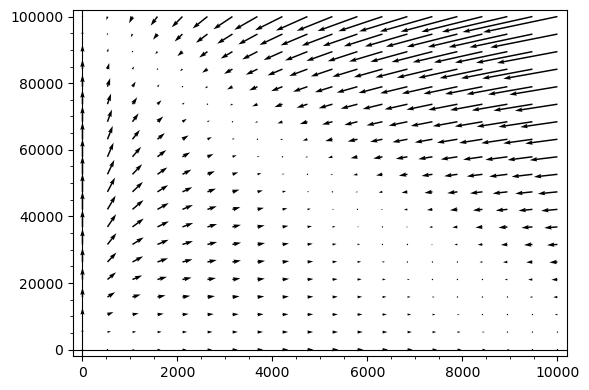
\includegraphics[width=\textwidth]{x0.png}
    \caption{equilíbrios de fronteira}
    \label{fig:my_label}
\end{figure}

\subsection{Estabilidade}

Os Equilíbrios $E_0$, $E_1$, $E_2$ e $\bar{E}$ representam um estado estacionário onde os herbívoros estão ausentes. A condição de estabilidade para esses equilíbrios são similares ao modelo de competição provado no modelo de Lotka-Volterra, que a taxa de morte de herbívoros, $Z$, excede o valor crítico $min(Z_i)$, dado por $Z_i=Y_1\eta_1(\textbf{n}_i)+Y_2\eta_2(\textbf{n}_i)$ com $n_1=(W_1,0)$, $n_2=(0,W_2)$ e $n_3=(\bar{n}_1,\bar{n}_2)$.\\
\begin{equation*}
\begin{aligned}
    \frac{dn_1}{dt} &= g_1 n_1 \left( 1 - \frac{n_1}{W_1} - \frac{\beta_{12}n_2}{W_1} \right) - \eta_1(\textbf{n})X\\
    \frac{dn_2}{dt} &= g_2 n_2 \left( 1 - \frac{n_2}{W_2} - \frac{\beta_{21}n_1}{W_2} \right) - \eta_2(\textbf{n})X\\
    \frac{dX}{dt}   &= Y_1\eta_1(\textbf{n})X+Y_2\eta_2(\textbf{n})X-ZX=[Y_1\eta_1(\textbf{n})+Y_2\eta_2(\textbf{n})]X-ZX
\end{aligned}
\end{equation*}
Isso é fácil de ver em $\frac{dX}{dt}$ pois se $Z>min(Z_i)$ essa derivada será negativa, o que acarreta na extinção dos herbívoros.

É de fácil visualização que $E_0$ é um equilíbrio instável, pois qualquer pequena variação não tende a voltar para ele, para $E_1$ teremos que é um equilíbrio localmente assintoticamente estável quando $\frac{\beta_{21}n_1}{W_2} > 1$, pois isso fará com que a derivada $\frac{dn_2}{dt}$ seja sempre negativa e $Z<Z_1$, para $E_2$ teremos que é um equilíbrio localmente assintoticamente estável quando $\frac{\beta_{12}n_2}{W_1} > 1$, pois isso fará com que a derivada $\frac{dn_1}{dt}$ seja sempre negativa e $Z<Z_3$ e para $\bar{E}$ teremos que é um equilíbrio localmente assintoticamente estável quando $\frac{\beta_{21}n_1}{W_2} < 1$ e $\frac{\beta_{12}n_2}{W_1} < 1$, com isso as derivadas vão depender dos valores de $n_1$ e $n_2$ para serem negativas ou positivas até se tornarem estáveis e $Z<Z_3$.

\subsection{Equilíbrios internos}

Devido a alta não linearidade das equações, é muito difícil obter uma solução analítico pro equilíbrio interior. Entretanto, podemos usar as raízes positivas das derivadas para determinar tal equilíbrio $(E^*)$. Utilizando o sistema de EDO's descrito em (8) temos:
\begin{align*}
    0=\frac{dX}{dt}&=\sum_{i=1}^2\left\{\frac{Y_ir_in_i}{1+t_{h_1}r_1n_1+t_{h_2}r_2n_2}\left[1-\frac{r_in_i}{4\frac{1}{2t_{h_i}}(1+t_{h_1}r_1n_1+t_{h_2}r_2n_2)}\right]\right\} - Z \\
    &=\sum_{i=1}^2\left[\frac{Y_ir_in_i}{1+t_{h_1}r_1n_1+t_{h_2}r_2n_2}-\frac{t_{h_i}Y_ir_i^2n_i^2}{2(1+t_{h_1}r_1n_1+t_{h_2}r_2n_2)^2}\right] - Z\\
    &=\sum_{i=1}^2\left[\frac{Y_ir_in_i[2(1+t_{h_1}r_1n_1+t_{h_2}r_2n_2)] - t_{h_i}Y_ir_i^2n_i^2}{2(1+t_{h_1}r_1n_1+t_{h_2}r_2n_2)^2}\right] - Z\\
    &=\sum_{i=1}^2\left[\frac{Y_ir_in_i(2+2t_{h_1}r_1n_1+2t_{h_2}r_2n_2-t_{h_i}r_in_i) }{2(1+t_{h_1}r_1n_1+t_{h_2}r_2n_2)^2}\right] - Z\\
    \implies \Upsilon_1(n_1^*,n_2^*)&=\sum_{i,j=1,i\neq j}^2\left[\frac{Y_ir_in_i^*(2+t_{h_i}r_in_i^*+2t_{h_j}r_jn_j^*) }{2(1+t_{h_1}r_1n_1^*+t_{h_2}r_2n_2^*)^2}\right] - Z=0\\
\end{align*}
e
\begin{align*}
    &\frac{dN_1}{dt}=g_1n_1\left(1-\frac{n_1+\beta_{12}n_1}{W_1}\right)-f_1(\textbf{n})X=0\\&\implies X=\frac{2(1+t_{h_1}r_1n_1+t_{h_2}r_2n_2)^2}{r_1n_1(2+t_{h_1}r_1n_1+2t_{h_2}r_2n_2)}g_1n_1\left(1-\frac{n_1+\beta_{12}n_1}{W_1}\right)\\
    &\frac{dN_2}{dt}=g_2n_2\left(1-\frac{n_2+\beta_{21}n_2}{W_2}\right)-f_2(\textbf{n})X = 0\\& \implies X=\frac{2(1+t_{h_1}r_1n_1+t_{h_2}r_2n_2)^2}{r_2n_2(2+2t_{h_1}r_1n_1+t_{h_2}r_2n_2)}g_2n_2\left(1-\frac{n_2+\beta_{21}n_2}{W_2}\right)
\end{align*}
igualando as duas equações
\begin{align*}
    &\frac{2(1+t_{h_1}r_1n_1+t_{h_2}r_2n_2)^2}{r_1(2+t_{h_1}r_1n_1+2t_{h_2}r_2n_2)}g_1\left(1-\frac{n_1+\beta_{12}n_1}{W_1}\right)=\frac{2(1+t_{h_1}r_1n_1+t_{h_2}r_2n_2)^2}{r_2(2+2t_{h_1}r_1n_1+t_{h_2}r_2n_2)}g_2\left(1-\frac{n_2+\beta_{21}n_2}{W_2}\right) \implies \\
    &(2+2t_{h_1}r_1n_1+t_{h_2}r_2n_2)g_1r_2\left(1-\frac{n_1+\beta_{12}n_1}{W_1}\right)=(2+t_{h_1}r_1n_1+2t_{h_2}r_2n_2)g_2r_1\left(1-\frac{n_2+\beta_{21}n_2}{W_2}\right) \implies\\
    &\Upsilon_2(n_1^*,n_2^*)= \sum_{i,j=1,i\neq j}^2 (-1)^j r_jg_i\left(1-\frac{n_i^*+\beta_{ij}n_i^*}{W_i}\right)(2+t_{h_j}r_jn_j^*+2t_{h_i}r_in_i^*) =0
\end{align*}

Se calcularmos a intercessão das curvas chegaremos nos pontos de equilíbrios interiores no plano $(n_1, n_2)$.

\newpage

\section{Discussão}

Utilizamos como base os modelos de competição de Lotka-Volterra, cuja equação para uma população de $N$ espécies é dada por 
\begin{align*}
    \frac{dn_i}{dt} = g_in_i\left( 1 - \frac{\sum_{j=1}^N \beta_{ij}n_j}{W_i} \right)
\end{align*}
e o modelo padrão Holling de tipo 2, com equação
\begin{align*}
    f(n) = \frac{n r}{1 + t_h n r}
\end{align*}
conseguimos expressar de maneira funcional o sistema proposto adicionando a variável de toxicidade aos sistemas já existentes. A partir das equações encontradas para a taxa de consumo $(f)$ e a taxa real de consumo ($\eta$), conseguimos um sistema de equações diferenciais que representa a relação planta-herbívoro no ambiente. \\

Seguimos o mesmo modelo utilizado em \cite{LI}, adicionando alguns detalhes que não estavam presentes nesse artigo, como passos não triviais omitidos nas equações e a utilização do \textit{SageMath9.3} para visualização dos 4 primeiros equilíbrios de fronteira. Tivemos foco no desenvolvimento passo a passo das equações obtidas, para uma melhor compreensão analítica do que ocorre a cada resultado encontrado.

\section{Conclusão}

Vimos com nossas análises que o fato de uma planta ter toxicidade influencia fortemente no desenvolvimento das equações e por consequência nos equilíbrios do sistema, pois torna ele mais realístico e diferente do Lotka-Volterra, mais comum nesse tipo de análise. Com possíveis análises futuras e modelos mais realistas usando dados coletados da natureza com herbívoros e plantas poderíamos chegar a melhores conclusões e gráficos mostrando a realidade de um sistema natural. Com isso poderíamos prever os riscos de determinada planta ou animal ser extinto de uma região e assim impedindo algumas extinções. 

\newpage

\bibliography{ref}
\bibliographystyle{ieeetr}



\end{document}
